% Todo:

\documentclass[12pt]{article}
\usepackage[no-math]{fontspec}	% no-math option required for accents package
\usepackage{hyperref}
\usepackage{xeCJK}
%\setCJKmainfont{SimSun}
\setCJKmainfont[BoldFont=SimHei,ItalicFont=KaiTi]{SimSun}
% \setCJKsansfont{SimHei}
% \setCJKmonofont{SimKai}
\setmainfont{Arial}

\usepackage{accents}		% for dots under Chinese for empahsis
\usepackage{cite}
\usepackage{graphicx}
\usepackage{float}
\usepackage{amsfonts}
% \usepackage{amsmath}	% for \tag
\usepackage{amssymb}	% for \multimap
% \usepackage{stmaryrd}
\usepackage{color}
%\usepackage[square,numbers]{natbib}
%\nocopyright
%\usepackage{latexsym,amsmath,amssymb,graphicx,hyperref}
%\usepackage{times} % gives you a bit more space if needed
\usepackage{titlesec}		% change color of section headings
\usepackage{verbatim}		% enables to define {comment} blocks
% \usepackage[most]{tcolorbox}		% color box
\usepackage{tikz-cd}		% commutative diagrams
\usepackage{enumerate}

% Left and right angle brackets
\makeatletter
\newsavebox{\@brx}
\newcommand{\llangle}[1][]{\savebox{\@brx}{\(\m@th{#1\langle}\)}%
  \mathopen{\copy\@brx\kern-0.5\wd\@brx\usebox{\@brx}}}
\newcommand{\rrangle}[1][]{\savebox{\@brx}{\(\m@th{#1\rangle}\)}%
  \mathclose{\copy\@brx\kern-0.5\wd\@brx\usebox{\@brx}}}
\makeatother

% Make dots under Chinese characters for emphasis
\renewcommand{\d}[1]{$\underaccent{\scalebox{0.7}{\textbullet}}{\textrm{#1}}$}
\makeatletter\newcommand{\ds}[1]{\@tfor\next:=#1\do{\d{\next}}}\makeatother

\titleformat{\section}
{\color{blue}\normalfont\Large\bfseries}
{\color{blue}\thesection}{1em}{}
\titleformat{\subsection}
{\color{blue}\normalfont\large\bfseries}
{\color{blue}\thesubsection}{1em}{}

\renewcommand\abstractname{\textcolor{blue}{Abstract}}

\definecolor{LogicColor}{rgb}{0.4,0.1,0.4}  % Magenta
\definecolor{Hilight}{rgb}{0.9,0.9,0.8}  % yellow
\definecolor{grey}{rgb}{0.9,0.9,0.9}  % grey
% \definecolor{LogicColor}{rgb}{0,0,0}	% for black-and-white paper

\newcommand{\concept}[1]{\textbf{\textcolor{blue}{#1}}}

\newcommand{\english}[1]{\rmfamily \textit{``#1''}\rmfamily}
\newcommand{\formula}[1]{\textcolor{LogicColor}{#1}}

\newcommand{\hilight}[1]{\begin{tcolorbox}[breakable]#1\end{tcolorbox}}

\newcommand{\tab}{\hspace*{1cm}}

\newcommand*\sigmoid{\vcenter{\hbox{
\includegraphics{sigmoid.png}}}}
\newcommand*\sadface{
\includegraphics[scale=0.25]{face-sad.png}}
\newcommand*\smiley{
\includegraphics[scale=0.5]{smiley.jpg}}

\setlength{\oddsidemargin}{1cm}
\setlength{\evensidemargin}{1cm}
\setlength{\textwidth}{14cm}

\linespread{1.2}

\title{\textcolor{blue}{Genifer 5.3 theoretical notes}}
\author{YKY (\textit{甄景贤})}
%% \date{30 June 2015}
%% \institute{}

\begin{document}

%\tab\tab\tab \parbox{9cm}{\textit{筌者所以在鱼,得鱼而忘筌;蹄者所以在兔,得兔而忘蹄;言者所以在意,得意而忘言。}}
% \vspace{-0.5cm}
%\begin{flushright}
%\textemdash\, 
%\textit{《庄子 $\cdot$ 外物》} \hspace*{2cm}
%\end{flushright}

% \sffamily

{\let\newpage\relax\maketitle}

\maketitle
\setlength{\parindent}{0em}
\setlength{\parskip}{2.5ex plus0.5ex minus1.2ex}

\section{Top-level architecture}

在最高层面上,RL 控制 RNN:

\begin{center}
\fbox{\parbox[b][][t]{3.2em}{RL \\
\fbox{\parbox[c][][s]{2.2em}{RNN} }
} }
\end{center}

可以想像,RNN 是 RL 的 ``mental model''; 换句话说,我们的 RL 比普通 RL 有更复杂的内部模型。

馀下的工作是,定义 RL 的四个元素: states, actions, rewards, policy。

\section{Unification of RL and RNN}

在统一 RL 和 RNN 的时候,我发现它们之间的关系非常简单:

从\textbf{强化学习}的角度来看,我们需要学习的是这个 policy 函数:
\begin{center}
\begin{tikzcd}[row sep=tiny]
\mbox{policy : ~~state} \arrow[r, mapsto, "\scalebox{0.8}{action}"] & \mbox{state'}
\end{tikzcd}
\end{center}
而 $K$ 可以看成是我们的 mental state,那么 RL 的 action 就是将 $K$ 变成 $K'$ 的作用,而那正是 $D$!
\begin{center}
\begin{tikzcd}[row sep=tiny]
K \arrow[r, mapsto, "\scalebox{1.3}{$D$}"] & K'
\end{tikzcd}
\end{center}
换句话说,$D$ 就是 policy。

从强化学习的角度看,某些推导过程的结果,可以给予奖励:
\begin{center}
\begin{tikzcd}[row sep=tiny]
K_0 \arrow[r, mapsto, "\scalebox{1.3}{$D^n$}"] & K_\bot \quad \updownarrow \bigstar
\end{tikzcd}
\end{center}
$\updownarrow \bigstar$ 的意思是「给予正或负奖励」。  我们要学习的是 $D$ 也就是 policy。  学习算法的基础是著名的 Bellman optimality condition (见下节)。

但 $D$ 本身是 RNN,它还可以透过 back-prop 进行学习,两者似乎是不同的。  Back-prop 是透过 $\frac{\partial}{\partial D} \mbox{~error}$ 的梯度来学习。

以下我们分别讲述 4 种学习模式:
\begin{itemize}
\item 学习~听/讲
\item RL-based learning
\item inductive learning
\end{itemize}

\section{Bellman equation}

回顾一下 Bellman equation 是:
$$ U(S) = \max_a \{ R(S,a) + \beta U(S') \}$$
其中 $U$ = utility, $R$ = reward, $\beta$ = discount factor, $a$ = action, $S \stackrel{a}{\longrightarrow} S'$。 它是一条 recursive equation,表示本状态的最佳效用,是下一状态的效用,加上本状态的 reward,再取最优化。

\begin{center}
\colorbox{grey}{\parbox{0.95\textwidth}{\setlength{\parskip}{2.5ex}
这个方程有\textbf{微分版本},叫 Hamilton-Jacobi equation。 假设:
$$ U(x,t) = \min_u \{ \int_t^{t'} C(x,u)dt + U(x',t') \} $$
其中 $t$ 是时间,$u$ 是 control parameters,$C$ 是 cost-rate function:
$$ \int C dt = R = \mbox{reward} $$
这个积分表示「路径中的 cost」,$U(x',t')$ 是「终点的 cost」。

这条方程写成微分形式就是 Hamilton-Jacobi equation:
$$ \frac{d}{dt} U(x,t) = \min_u \{ C(x,u) + \nabla U(x,t) \cdot f(x,u) \} $$
而 $x$ 必需遵从:
$$ \dot{x}(t) = f(x(t),u(t)) $$
这个方程的的形式很接近量子力学中的 Schr\"{o}dinger equation:
$$ i \hbar \frac{\partial}{\partial t} \Psi(x,t) = \left[ V(x,t) + \frac{-\hbar^2}{2\mu} \nabla^2 \right] \Psi(x,t) $$
$\Psi$ 类似於我们的 $U$(可能它是一个自然界想 minimize 的东西?)
}}
\end{center}

在思维过程中,除了结果以外,其他步骤是没有奖励的,所以 reward 只可以是一个微小的负常数(代表时间损耗)。 在这情况下 Bellman 算法可能变到和 back-prop 差不多甚至一样,但我还未详细验算。

\section{学习~听/讲}

我发现~听/讲~是可以靠 RL 学习的。

Learning modes:
\begin{enumerate}
\item Listening:  $K$ contains understanding of linguistic input, test $K$
\item Speaking:  $K$ is known, $\mbox{output} \approx_{L} K$
\end{enumerate}

\begin{center}
\begin{tikzcd}[row sep=tiny]
K_0 \arrow[r, mapsto, "\scalebox{1.3}{$D^n$}"] & \mbox{输出句子} \quad \updownarrow \bigstar
\end{tikzcd}
\end{center}

\section{RL-based learning}



\section{Inductive learning}

Actions:
\begin{enumerate}[(A)]
\item deduction (apply $D$)
\item write / add to $K$ partially:  $K := K'$ or $K \mbox{+=} K'$
\item learn = change $D$
\item learn = neurogenesis
\end{enumerate}


%%%%%%%%%%%%%%%%%%%%%%%%%%%%%%%%%%%%%%%%%%%%%%%%%%%%%%%%%%%%%%%%%%%%%%%%
{\color{red}\rule{10cm}{2pt}}

上次的模型:
\begin{figure}[H]
\centering
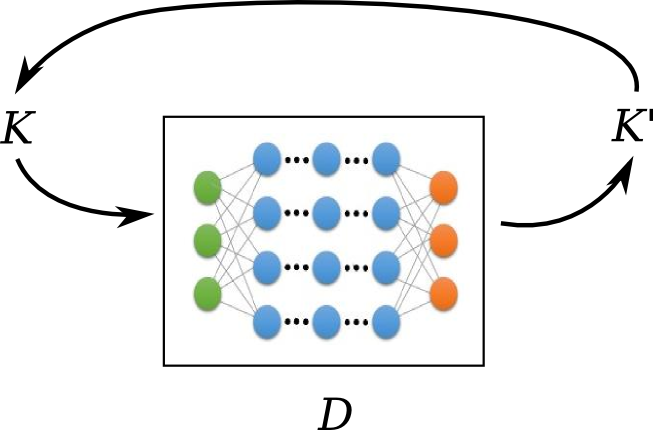
\includegraphics[scale=0.75]{reasoner-model.png}
\end{figure}
$K$ 可以直接输出一些 words,words 的序列构成句子。

这做法太简单,因为我假设自然语言是一些 sequences,但自然语言的结构不是序列那么简单,例如「未吃过饭」包含「吃过饭」的序列,但语义是相反的。 所以自然语言必须要在语义 (semantic) 层面上处理,而不是语法 (syntactic) 层面上。 自然语言的复杂性是不会轻易消失的。

\section{Language map}

在 Memory Networks\cite{Weston2015} 里,他们用了一个 language map,将自然语言句子转换成 internal representation of knowledge in $\mathbf{K}$,$\mathbf{K} \ni K$ 是知识状态的空间。 可以叫这个 map 做 language map:
\begin{eqnarray}
\mathcal{L} :& \mathbf{S} & \rightarrow \mathbf{K} \nonumber \\
\mathcal{L} :& \mbox{句子} & \mapsto K \nonumber
\end{eqnarray}
(但其实句子只是知识状态 $K$ 的一部分。)

於是我们的 RNN model 变成这样:
\begin{center}
\begin{tikzcd}%[column sep=small]
\mbox{句子输入}\arrow[r,"\scalebox{1.3}{$\mathcal{L}$}"] & \mathbf{K} \arrow[r,"\scalebox{1.3}{$\mathcal{L}^{-1}$}"] \arrow[loop,"\scalebox{1.3}{$D$}",swap,looseness=4] & \mbox{句子输出}
% S\arrow{r} & K\arrow{r}\arrow{r}{loop,"D"} & S
\end{tikzcd}
\end{center}
%$$ \mbox{句子输入} \stackrel{\mathcal{L}}{\longrightarrow} \stackrel{\stackrel{\mbox{\raisebox{3pt}{\normalsize{$D$}}}}{\raisebox{5pt}{\scalebox{2.0}{\ensuremath{\rotatebox[origin=c]{180}{$\circlearrowleft$}}}}}}{\mathbf{K}} \stackrel{\mathcal{L}^{-1}}{\longrightarrow} \mbox{句子输出} $$

有了这个 language map 是很方便的,但它有几个问题:
\begin{itemize}

\item 需要用到 NLP parsing,很麻烦,如果能省略比较好

\item 这个 map 基本上 fix 了 internal knowledge representation 的形式。 但我的直观(也可能错误)觉得 knowledge representation 应该是「不知道的」比较好,它应该是由学习 $D$ 的过程「诱导」出来的,换句话说: the knowledge representation format should be \textit{induced} from the learning of $D$.  因为以前在经典逻辑系统中,$K$ = KB (knowledge base) 是一些命题的集合,换句话说 $ K = \bigsqcup S_i $,$S_i$ 是句子或「命题」。  当时的做法是将 KB 组织成 hierarchical 结构,方便搜寻。 但我觉得如果 $\mathbf{K}$ 的结构是这样的话,跟原问题的情况太相似,一切都太「有秩序」,可能不是神经网络最有效的用法。

\item 自然语言是需要慢慢「吸收」或「理解」(comprehend) 的,但这过程在 Memory Networks 的模型里忽略了。  将自然句子转换成 logical 形式(即 internal representation),几乎是不需时间的 transliteration 过程。  如果输入一本《世界历史》的原文,不消一秒便可以转换成 internal representation,但不能说 Genifer 已经「理解」了全书的内容吧?

\end{itemize}

\section{理解 / 慢吸收}
% \label{language-comprehension}

所以 $\mathcal{L}$ 不是一个普通 map 而是一个很复杂的\ds{过程}。

对新输入知识的「慢吸收」包括这些运作:
\begin{itemize}
\item consequences (找出新命题的所有可能推论结果,至少在 $n$ 步之内)
\item consistency (新信念不和旧信念抵触)
\item explanations (新信念可以被已有知识解释)
\end{itemize}

「理解」的过程可以看成是: 经过 $n$ 次的推导 $\mathcal{D}$,$K$ 变成 $K'$:
\begin{center}
\begin{tikzcd}[row sep=tiny]
K \arrow[r, mapsto, "\scalebox{1.3}{$D^n$}"] & K'
\end{tikzcd}
\end{center}
% $$ K \stackrel{D^n}{\mapsto} K' $$
而 $K'$ 有我们想要的特性(即「后果、和谐、解释」)。  问题就是怎样测试 $K'$ 有这些特性?  特别困难的原因是 $K' \in \mathbf{K}$ 的 representation 是\ds{不透明}的。

$K'$ 的特性可以怎样测试?

似乎唯一的方法是透过这样的查询:
\begin{center}
\begin{tikzcd}[row sep=tiny]
K \arrow[r, mapsto, "\scalebox{1.3}{$D^n$}"] & Q \; ?
\end{tikzcd}
\end{center}
% $$ K \stackrel{D}{\longrightarrow} .... \; q \; ? $$
但 $Q$ 也是 $\in \mathbf{K}$,而 $\mathbf{K}$ 的结构是不透明的。

如果有 $\mathcal{L}$ 的话,直接将问题用自然语言问,变成 $Q = \mathcal{L}(\mbox{句子})$,就可以查询 $K$。 换句话说,$\mathcal{L}$ 的好处是容许 direct access to $K$,将知识状态的内容,直接用自然语言读出来(或写入去)。 但现实中不存在一个简单的 $\mathcal{L}$ map。

$\mathcal{L}$ 不存在,找不到 $Q$ 用来查询 $K$。 

\section{Speech generation (发言)}

如果 Genifer 学会「说话」,就等於查看 $K$ 的内容。 但说话不等於将所有知识状态的内容「和盘托出」,而是有两种模式:
\begin{itemize}
\item 查询某句子 $S_{query}$ 是不是真的
\item 查询关於某题目 $S_{interest}$ 的内容,eg: "Tell me about your mother"
\end{itemize}
但这两个动作都要求有某种办法将 $query$ 或 $interest$ 映射到 $\mathbf{K}$ 的某个「位置」,而这正是我们没有的。

「说话」本身是一个复杂的算法,它不是一个简单的映射,而是需要用 $D$ 思考的运作。

无论是「理解」或「说话」,都是复杂算法,而且 $\mathbf{K}$ 是不透明的。  表面上似乎没有希望,但神经网络的好处是: \ds{可以同时学习两个过程},即使这两个过程\ds{互相依赖}。

\section{学习}

为了方便思考,现假设有 $\mathcal{L}$,容易做到以下两种学习方式:

\subsection{Inductive learning}

举例:\\
\tab 小明是香港人 $\wedge$ 小明戴眼镜 \\
\tab 小强是香港人 $\wedge$ 小强戴眼镜 \\
\tab 小雄是香港人 $\wedge$ 小雄戴眼镜 \\
\tab 小娟是香港人 $\wedge$ 小娟戴眼镜 \\
\tab 结论: 所有香港人都戴眼镜 \\
用逻辑表示这法则就是:
$$ \forall X. \; \mbox{Hong-Kong}(X) \Rightarrow \mbox{wear-glasses}(X) $$
但在 RNN 里,这法则是暗含在 $D$ 之中。 例如如果 $k = \mbox{「大强是香港人」}$,那么 $D$ 作用在 $K$ 上最终会得出 $K' = \mbox{「大强戴眼镜」}$。

换句话说,已知 $K_0$,$K^*$,学习 $D$:
$$ K_0 \stackrel{D}{\longrightarrow} .... \; K^* $$

因为我们可以用 $K = \mathcal{L}(\mbox{自然语言句子})$ 来计算 $K_0$ 和 $K^*$,所以这个算法是可行的。

\begin{comment}
%===========================================================================
\section{RNN}

整个 Genifer 系统包含 RL + RNN 两部分。

RNN ($D$) 是一个 feedforward NN,只是它的输出再回溃到输入。


它可以执行 3 个运作:

\subsection{Deduction}

Deduction 只需要 forward propagation。  (实际上 deduction 可能没有什么用,重要的是 querying。)

\subsection{Learning}

Learning 是通过 back-prop,我们要求的是从 $K_0$ 开始:
\begin{eqnarray}
K_0 \stackrel{D}{\longrightarrow} .... \; K_\infty \nonumber \\
K_\infty \ge K^*
\end{eqnarray}
但这里需要用到 $\ge$ 关系,下述。

目的是学习 $D$,令误差 $\mathcal{E}$ 最少。

梯度 $\frac{\partial \mathcal{E}}{\partial W}$ 的计算应该是可行的; 这里 $W$ 是 RNN 的 weights。

但怎样计算 $\mathcal{E} = K_\infty - K^*$ ?  有个严重问题是: 我们要知道 $K^*$ 的知识的表达方式,但如果 $D$ 是个 black box,$K^*$ 的 representation 就不是透明的。

Joseph 找到一篇 paper,叫 Memory Networks,来自 Facebook AI research \cite{Weston2015}。 他们也是用 RNN 来学习 Q\& A,但它有一个 component $I$ = input feature map,负责将句子变成 internal feature representation,它需要涉及传统 NLP 的 parsing。 我们可不可以不做这步? \sadface

问题是如果输出是 words,我们必须比较句子,亦即是 $K$ 的\textbf{序列}。 似乎可以用 convolution 方法: 记 $S := K_0, K_1, K_2, ....$ 为输出的 sequence,$S^* := K^*_0, K^*_1, ..., K^*_m $ 为想要的答案 sequence,则误差可以定义成:
$$ \mathcal{E} := S * S^* $$
其中 $*$ 是 convolution。 (但我不是 100\% 肯定这个用法是否正确。)

\subsection{Querying}

\begin{eqnarray}
K_0 \stackrel{D}{\longrightarrow} .... \; K_\infty \nonumber \\
K_\infty \ge ? \; K^*
\end{eqnarray}

传统逻辑的做法是,找 $K_n$ ($n$ 个推导步骤之后的结果),然后试试 $K_n$ 包不包含 $K^*$。 但通常更有效率是反向地由结论 $K^*$ 开始寻找。

可以看成是这个问题:
\begin{eqnarray}
\mbox{solve}\quad\quad D^n(\mathbf{x}) & > & K^* \nonumber \\
K_0 & \ge & \mathbf{x}
\end{eqnarray}
其中 $\mathbf{x}$ 是变量。 我们要求 $>$ 是大於某个 threshold $\epsilon$。  这是一条 iterative equation,似乎还有希望。

上次说过如果 D 是 monotonous,即 $\forall \mathbf{x} \; D(\mathbf{x}) \ge \mathbf{x}$,可能有帮助。

\subsection{\texorpdfstring{$\ge$}{>} 关系}

$\ge$ 是逻辑中的「generalize」关系,它有两种模式:
\begin{itemize}
\item 人会死 $\ge$ Socrates 会死
\item 人会死 $\ge$ ( 人会死 $\wedge$ 月亮是圆的 ~)
\end{itemize}

在 (topological) vector space 理论里,我们可以定义 vector 之间的 $\mathbf{v}_1 \ge \mathbf{v}_2$,方法是选取任何一个 cone (锥形)$C$:
$$ \mathbf{v}_1 \ge \mathbf{v}_2 \Leftrightarrow (\mathbf{v}_1 - \mathbf{v}_2) \in C $$
例如如果在平面上,$C$ 可以是右上角的 quadrant。

我在考虑: 我们可不可以选取任何一个在 $\mathbf{K}$ 空间中的 cone 来定义 $\ge$,然后让 RNN 自己学习 $\ge$ 的逻辑结构(例如~ 动物 $\ge $ 猫、$A \ge A \wedge B$)?

\section{RL}

整个 Genifer 系统会是这样的:
\begin{figure}[H]
\centering
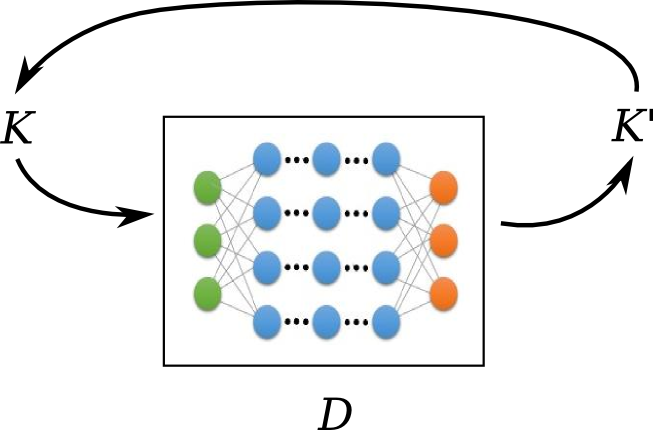
\includegraphics[scale=0.75]{genifer-model-0.png}
\end{figure}

设计一个 RL 系统只需定义 4 个元素: \{ 状态 (states)、行动 (actions)、奖励 (rewards)、方案 (policy) \},其中 policy 是由算法自动计算出来的 states $\rightarrow$ actions 函数。

可以想像 RL 控制一个婴儿慢慢~\ds{调教}她的四肢动作,最后学会走路,这是经典的 RL 应用。

但在 Genifer 中,reasoner 是 Genifer 的一部分,它教导 Genifer 如何思考,但它本身受 RL 控制。

要小心避免 recursive 谬误: 对 RL 来说,reasoner 是一个 external 物体,换句话说,reasoner 虽然是一个导师,但它的内部是\ds{透明的},这个导师本身可以被 RL 调教。

要小心区分 Genifer 的 actions:
\begin{itemize}
\item 她对外部世界的 actions,例如「举手」、「小便」
\item 她对 reasoner 的 \textit{control actions}
\end{itemize}

上次说过,reasoner 只有3个基本动作: 推导、学习、查询。  如果只能调教这3个 actions,则 RL 的作用不大,所以要将 reasoner 的运作「精细化 (refine)」。

方法是: RL 的 control actions 可以直接改写状态 $K$ 的内容。 例如说:『现在紧急状态,要小便』,那么 Genifer 可能会停下现时的工作,去厕所。

$K$ 的内容基本上是无限制的,所以可以有近乎无限的 actions。 在经典 RL 里,通常用一个 table 记录所有 state-action transitions,但在这情况下我们必须用 function approximation 去近似这个 table,这也没有大碍。 

\section{Remaining problems}

\section{慢吸 (slow absorption)}

第一个问题是,为什么需要慢慢「吸收」句子?
\begin{itemize}
\item 找出与其他句子的关系
\item 逻辑和谐
\item 找出句子下游的逻辑后果
\item 最后,找出最适当的在句子空间中的位置
\end{itemize}

慢吸需要服从的约束是?
\begin{itemize}
\item fast
\item accurate
\item comprehensive (全面)
\end{itemize}
全面的意思是: 在一定复杂性以下可以推导到的结论,就应该推导到(这涉及 $P =? NP$ 问题)。

现在我们似乎只剩下 $G$ 的结构可以改变。 单单改变 G 是否可以达到「更快、更准、更全面」?

%===========================================================================
\end{comment} 

% \section*{Acknowledgments}

\bibliographystyle{plain} % or number or aaai ...
\bibliography{AGI-book}

\end{document}
